\chapter{Les clients}
Les clients sont le cœur de l'application, elle a donc besoin d'ajouter de nouveau clients pour pouvoir être utilisée. 
\begin{figure}[H]
	\centering
	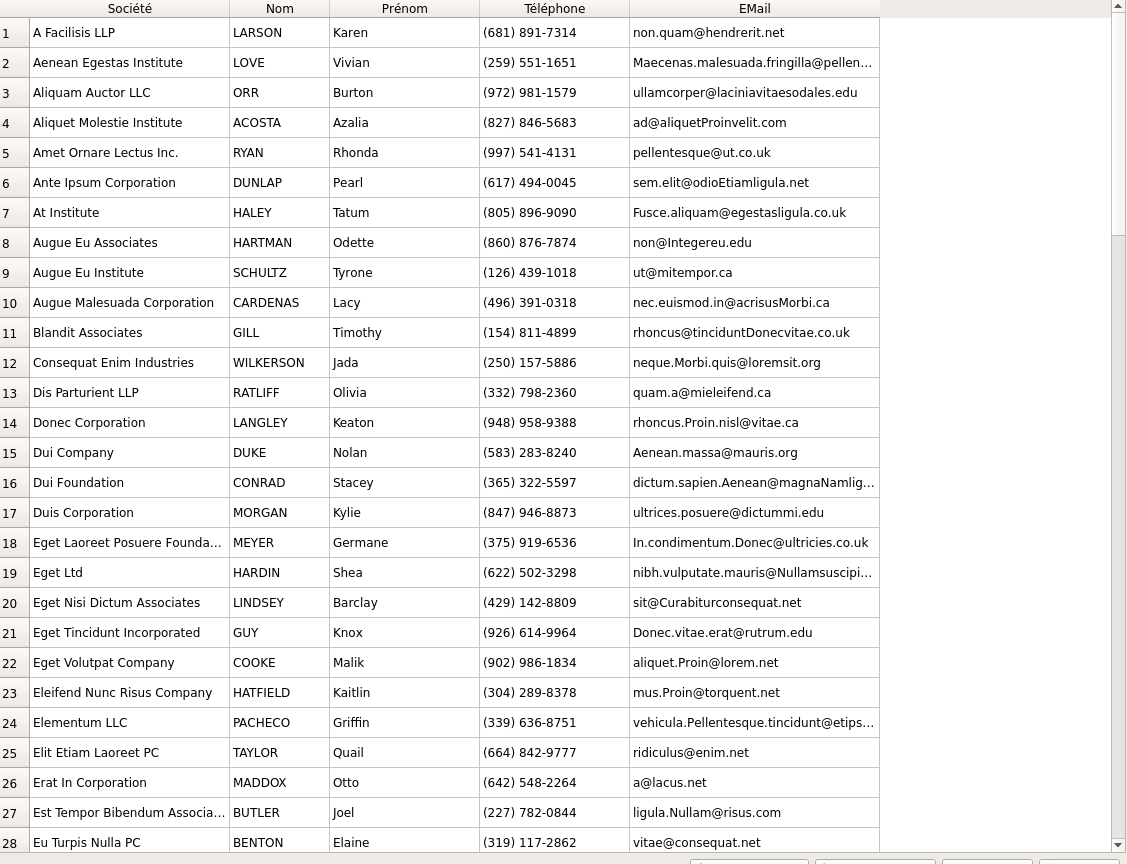
\includegraphics[width=12cm]{screens/clients.png}
	\caption{Gestion des clients}
\end{figure}

\section{Liste des clients\index{Client!Liste}}
La liste des clients, cf. figure 3.1, est accessible dès l’ouverture du logiciel. Celle-ci se trouve au centre du logiciel. 

La liste des clients contient uniquement les informations permettant de facilement les identifier à savoir, le nom de la société, le nom,
prénom, le numéro de téléphone et l’adresse e-mail. La sélection dans le tableau de l’un des clients permet, via le panneau du client,
d’obtenir les informations détaillées sur celui-ci. 

\section{Ajout d'un client\index{Client!Ajouter}}
L'ajout d’un patient peut se faire soit via le menu <<Client $\rightarrow$ Nouveau Client>>, via la barre d'outils ou encore via le bouton situé sous la
liste. 
\begin{figure}[H]
	\centering
	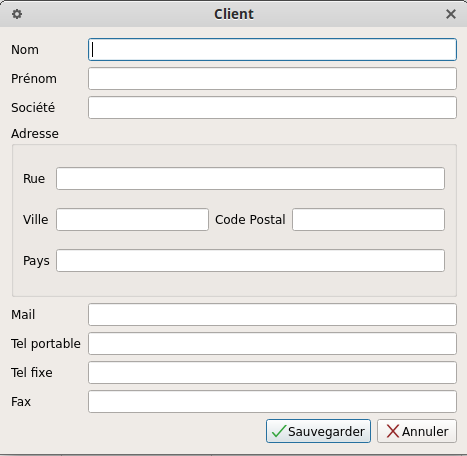
\includegraphics[width=7cm]{screens/ajouterClient.png}
	\caption{Ajouter un client}
\end{figure}

\section{Édition d'un client\index{Client!Éditer}}
L’édition d’un client a pour but de corriger d’éventuels erreurs sur les informations d’un client. Pour ce faire, il suffit de sélectionner
un client dans le tableau et de cliquer sur le bouton <<Modifier>> situé sous la liste des clients ou, via le menu contextuel, lors d’un clic
droit sur le client dans le tableau. 
 La fenêtre est similaire à celle lors d’un ajout de client, seul diffère les champs qui sont déjà pré-remplis. 

